\documentclass[twoside]{article}
\author{Michele Mazza}
% Pacchetti di Codifica e Lingua
\usepackage[utf8]{inputenc}
\usepackage[T1]{fontenc}
\usepackage[italian]{babel}

% Pacchetti Grafici e Diagrammi
\usepackage{graphicx}
\usepackage{tikz}
\usepackage{tikz-3dplot}
\usetikzlibrary{angles,quotes,arrows.meta, positioning, 3d, matrix, calc}
\usepackage{pgfplots}
\pgfplotsset{compat=1.18}

% Pacchetti Matematici
\usepackage{amsmath, amssymb}

% Scegliere tra amsthm e ntheorem
%\usepackage{ntheorem}
% Se si preferisce amsthm, commentare la riga sopra e decommentare la seguente
\usepackage{amsthm}
\usepackage{cancel}

% Pacchetti per Tabelle e Unità di Misura
\usepackage{geometry}
\usepackage{siunitx}
\usepackage{booktabs}
\usepackage{tabularx}
\usepackage{colortbl}
\usepackage{adjustbox}

% Pacchetti per Layout e Formattazione
\usepackage{fancyhdr}
\usepackage{float}
\usepackage{microtype}
\usepackage{multicol}

% Altri Pacchetti Utili
\usepackage{mdframed}
\usepackage{animate}
\usepackage{ulem}
\usepackage{eurosym}

% Pacchetto enumitem
\usepackage{enumitem}

% Definizioni dei Colori e Comandi Personalizzati
\definecolor{lightblue}{HTML}{9cd8fc}
\definecolor{myblue}{HTML}{139FE9}
\definecolor{myblack}{HTML}{303030}
\definecolor{mygray}{HTML}{787878}
\definecolor{mywhite}{HTML}{c7c7c7}
\newcommand{\norm}[1]{\left\lVert#1\right\rVert}

% Ambienti Personalizzati
% Usa \theoremstyle e \theorembodyfont come necessario
\newmdtheoremenv[
    backgroundcolor=orange!10,
    linecolor=myblue,
    linewidth=0pt,
    leftmargin=0pt,
    rightmargin=0pt,
    innerleftmargin=10pt,
    innerrightmargin=10pt,
    innertopmargin=10pt,
    innerbottommargin=10pt,
    nobreak
]{curiosity}{Curiosità}

\newmdtheoremenv[
    font=\normalfont\small,
    linewidth=0pt,
    innerleftmargin=10pt,
    innerrightmargin=10pt,
]{example}{Esempio}

\newmdtheoremenv[
  backgroundcolor=lightblue,
  linecolor=myblue,
  linewidth=1.5pt,
  innertopmargin=10pt,
  innerbottommargin=10pt,
  innerrightmargin=10pt,
  innerleftmargin=10pt,
  nobreak
]{theorem}{Teorema}

\newmdtheoremenv[
  backgroundcolor=gray!10,
  linewidth=0pt,
  innertopmargin=-5pt,
  innerbottommargin=5pt,
  innerrightmargin=10pt,
  innerleftmargin=10pt,
  nobreak
]{definition}{Definizione}

\newmdtheoremenv[
  backgroundcolor=gray!10,
  linecolor=myblue,
  linewidth=1.5pt,
  innertopmargin=-5pt,
  innerbottommargin=5pt,
  innerrightmargin=10pt,
  innerleftmargin=10pt,
  nobreak
]{proposition}{Proposizione}


% Configurazioni di fancyhdr
\pagestyle{fancy}
\fancyhf{}
\fancyhead[RE,RO]{\nouppercase{\rightmark}}
\fancyfoot[C]{\thepage}
\renewcommand{\headrulewidth}{0.0pt}
\renewcommand{\footrulewidth}{0pt}
\geometry{a4paper, left=20mm, right=20mm, top=20mm, bottom=20mm}

\usepackage{titlesec} % Pacchetto per personalizzare i titoli delle sezioni

% Definisci i colori per le diverse sezioni
\titleformat{\section}
{\color{black}\normalfont\Large\bfseries}
{\thesection}{1em}{}

\titleformat{\subsection}
{\color{red}\normalfont\large\bfseries}
{\thesubsection}{1em}{}

\titleformat{\subsubsection}
{\color{blue}\normalfont\normalsize\bfseries}
{\thesubsubsection}{1em}{}

% Pacchetti Aggiuntivi
\usepackage{xparse,array}

% Pacchetto Hyperref (inserito per ultimo)
\usepackage{hyperref}

\begin{document}
\title{Analisi T-B}
\maketitle
\hrulefill
\section{Rn euclideo, topologia, limiti e continuità}
\subsection{Operazioni tra vettori}
\subsubsection{Modulo o norma}
Sia \(\vec{x} \in \mathbb{R}^n\), scriviamo \(\vec{x} = (x_1, x_2, \ldots, x_n)\) con \(x_i \in \mathbb{R}\).\\
Chiamiamo \textbf{norma} o \textbf{modulo} di \(\vec{x}\) il numero reale non negativo
\begin{equation}
  \boxed{\norm{\vec{x}} = \sqrt{\sum_{i=1}^{n} x_i^2} =\sqrt{x_1^2 + x_2^2 + \ldots + x_n^2}}
\end{equation}
Essa rappresenta la lunghezza del vettore \(\vec{x}\) nello spazio euclideo \(\mathbb{R}^n\).
\subsubsection{Versore}
Chiamiamo \textbf{versore} di \(\vec{x}\) il vettore
\begin{equation}
  \boxed{vers\ \vec{x} = \frac{\vec{x}}{\norm{\vec{x}}}, \quad \text{se} \quad \vec{x} \neq \vec{0}}
\end{equation}
\begin{figure}[H]
  \centering
  \tdplotsetmaincoords{70}{120}
  \begin{tikzpicture}[tdplot_main_coords, scale=0.5]
    % valori massimi degli assi cartesiani
    \def\xMax{7}
    \def\yMax{7}
    \def\zMax{4}
    % a
    \def\ax{7}
    \def\ay{7}
    \def\az{7}
    % b
    \def\bx{3}
    \def\by{3}
    \def\bz{3}
    % c
    \def\cx{0}
    \def\cy{0}
    \def\cz{3}
    \draw[-latex, thick] (-\xMax,0,0) -- (\xMax,0,0) node[anchor=north east]{\(x\)};
    \draw[-latex, thick] (0,-\yMax,0) -- (0,\yMax,0) node[anchor=west]{\(y\)};
    \draw[-latex, thick] (0,0,-\zMax/2) -- (0,0,\zMax) node[anchor=south]{\(z\)};
    \draw[fill=mygray, opacity=0.05] (-\xMax,-\yMax,0) -- (\xMax,-\yMax,0) -- (\xMax,\yMax,0) -- (-\xMax,\yMax,0) -- cycle;
    \draw[-stealth, ultra thick, blue] (0,0,0) -- (\ax,\ay,\az) node[anchor=north west]{\(\vec{x}\)};
    \draw[-stealth, ultra thick, red] (0,0,0) -- (\bx,\by,\bz) node[anchor=north west]{\(vers\ \vec{x}\)};
  \end{tikzpicture}
\end{figure}
\subsubsection{Base canonica}
\'E detta \textbf{base canonica} di \(\mathbb{R}^n\) l'insieme di $n$ vettori
\begin{equation}
  \boxed{
    \begin{matrix}
      \vec{e}_1 = (1, 0, 0, \ldots, 0) \\
      \vec{e}_2 = (0, 1, 0, \ldots, 0) \\
      \vdots                           \\
      \vec{e}_n = (0, 0, 0, \ldots, 1)
    \end{matrix}}
\end{equation}
così possiamo scrivere un generico vettore \(\vec{x} \in \mathbb{R}^n\) come combinazione lineare dei vettori della base canonica
\begin{equation}
  \boxed{\vec{x} = x_1\vec{e}_1 + x_2\vec{e}_2 + \ldots + x_n\vec{e}_n = \sum_{i=1}^{n} x_i\vec{e}_i}
\end{equation}
Ricordiamo che
\begin{itemize}
  \item \textbf{Prodotto per uno scalare}
        \begin{equation*}
          \boxed{\lambda \cdot \vec{x} = \lambda \cdot \vec{x}}
        \end{equation*}
        \begin{equation*}
          \boxed{\lambda \cdot \vec{x} = \lambda \cdot (x_1, \ldots, x_n) = (\lambda \cdot x_1, \ldots, \lambda \cdot x_n), \quad \lambda \in \mathbb{R}}
        \end{equation*}
        \begin{figure}[H]
          \centering
          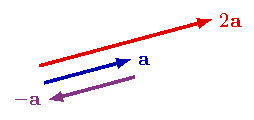
\includegraphics{src/vector/image10.pdf}
        \end{figure}
  \item \textbf{Somma}
        \begin{equation*}
          \boxed{\vec{x} + \vec{y} = \vec{z}}
        \end{equation*}
        \begin{equation*}
          \boxed{\vec{x} + \vec{y} = (x_1, \ldots, x_n) + (y_1, \ldots, y_n) = (x_1 + y_1, \ldots, x_n + y_n)}
        \end{equation*}
        \begin{figure}[H]
          \centering
          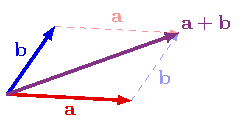
\includegraphics{src/vector/image3.pdf}
          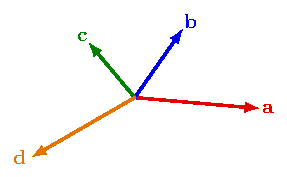
\includegraphics{src/vector/image4.pdf}
          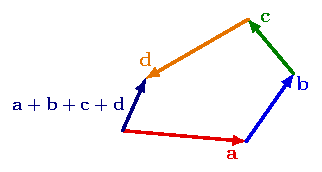
\includegraphics{src/vector/image5.pdf}
        \end{figure}
\end{itemize}
Così $\mathbb{R}^n$ ha una struttura di spazio vettoriale su $\mathbb{R}$.
\subsubsection{Vettori paralleli}
Dati due vettori \(\vec{x}, \vec{y} \in \mathbb{R}^n \setminus \{\vec{0}\}\), li diremo \textbf{paralleli} e scriveremo \(\vec{x} \parallel \vec{y}\) se
\begin{equation}
  \boxed{\lambda \vec{x} = \mu \vec{y}, \text{ per qualche } \lambda, \mu \in \mathbb{R} \setminus \{0\}}
\end{equation}
\subsubsection{Rappresentazione per componenti}
Nel caso in cui \(\mathbb{R}^n\) con \(n = 2, 3\), per le componenti di un vettore spesso scriveremo \((x, y)\) o \((x, y, z)\) per un generico vettore di \(\mathbb{R}^2\) o \(\mathbb{R}^3\) rispettivamente, e \(\vec{i}, \vec{j}\) o \(\vec{i}, \vec{j}, \vec{k}\) per la base canonica di \(\mathbb{R}^2\) o \(\mathbb{R}^3\) rispettivamente, quindi:
\begin{equation}
  \boxed{\vec{x} = (x,y) \in \mathbb{R}^2 = x\vec{i} + y\vec{j} \quad \lor \quad \vec{x} = (x,y,z) \in \mathbb{R}^3 = x\vec{i} + y\vec{j} + z\vec{k}}
\end{equation}
\begin{figure}[H]
  \centering
  \tdplotsetmaincoords{70}{120}
  \begin{tikzpicture}[tdplot_main_coords, scale=0.5]
    % valori massimi degli assi cartesiani
    \def\xMax{7}
    \def\yMax{7}
    \def\zMax{4}
    % a
    \def\ax{3}
    \def\ay{0}
    \def\az{0}
    % b
    \def\bx{0}
    \def\by{3}
    \def\bz{0}
    % c
    \def\cx{0}
    \def\cy{0}
    \def\cz{3}
    \draw[-latex, thick] (-\xMax,0,0) -- (\xMax,0,0) node[anchor=north east]{\(x\)};
    \draw[-latex, thick] (0,-\yMax,0) -- (0,\yMax,0) node[anchor=west]{\(y\)};
    \draw[-latex, thick] (0,0,-\zMax/2) -- (0,0,\zMax) node[anchor=south]{\(z\)};
    \draw[fill=mygray, opacity=0.05] (-\xMax,-\yMax,0) -- (\xMax,-\yMax,0) -- (\xMax,\yMax,0) -- (-\xMax,\yMax,0) -- cycle;
    \draw[-stealth, ultra thick, blue] (0,0,0) -- (\ax,\ay,\az) node[anchor=north west]{\(\hat{i}\)};
    \draw[-stealth, ultra thick, red] (0,0,0) -- (\bx,\by,\bz) node[anchor=south east]{\(\hat{j}\)};
    \draw[-stealth, ultra thick, orange] (0,0,0) -- (\cx,\cy,\cz) node[anchor=west]{\(\hat{k}\)};
  \end{tikzpicture}
\end{figure}
\subsubsection{Prodotto scalare}
Se \(\vec{u}\) e \(\vec{v}\) sono due vettori di \(\mathbb{R}^n\), definiamo \textbf{prodotto scalare} di \(\vec{u}\) e \(\vec{v}\) il numero reale
\begin{equation}
  \boxed{\vec{u} \cdot \vec{v} = \left(\vec{u}, \vec{v}\right) = u_1v_1 + \ldots + u_nv_n}
\end{equation}
\begin{equation}
  \boxed{\vec{u} \cdot \vec{v} = \norm{\vec{u}} \cdot \norm{\vec{v}} \cdot \cos{\theta}}
\end{equation}
Misura l’allineamento tra due vettori calcolando la lunghezza del segmento proiettato di \(\vec{u}\) su \(\vec{v}\) moltiplicata per la lunghezza di \(\vec{v}\).\\
\textbf{Proprietà}
\begin{itemize}
  \item \(\vec{u} \cdot \vec{v} = \vec{v} \cdot \vec{u}\)
  \item \(\vec{u} \cdot \vec{v} = 0 \Leftrightarrow \vec{u} \perp \vec{v}\)
  \item \(\vec{u} \cdot \vec{u} = \norm{\vec{u}}^2\)
\end{itemize}
\begin{figure}[H]
  \centering
  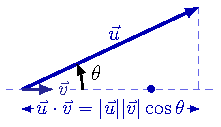
\includegraphics{src/vector/image11.pdf}
\end{figure}
\subsubsection{Angolo tra due vettori}
In \(\mathbb{R}^n\), si definisce \textbf{angolo} tra \(\vec{u}\) e \(\vec{v}\), entrambi non nulli, l'unico angolo \(\theta \in [0, \pi]\) tale che:
\begin{equation}
  \boxed{\cos{\theta} = \frac{\vec{u} \cdot \vec{v}}{\norm{\vec{u}} \cdot \norm{\vec{v}}}}
\end{equation}
\subsubsection{Prodotto vettoriale in R2}
\textbf{Per le matrici 2 x 2}
\begin{equation*}
  \vec{u} \times \vec{v} = det \begin{pmatrix}
    u_1 & u_2 \\
    v_1 & v_2
  \end{pmatrix}
\end{equation*}
\begin{equation*}
  \vec{u} \times \vec{v} = \quad \begin{tikzpicture}[>=stealth, baseline=-0.5ex]
    \matrix [
      matrix of math nodes,
      column sep=1em,
      row sep=1em
    ] (sarrus) {
      u_1 & u_2 \\
      v_1 & v_2 \\
    };
    \path[ultra thick]
    ($(sarrus-1-1.north west)-(0.5em,0)$) edge ($(sarrus-2-1.south west)-(0.5em,0)$)
    ($(sarrus-1-2.north east)+(0.5em,0)$) edge ($(sarrus-2-2.south east)+(0.5em,0)$);
    \path[thick]
    (sarrus-1-1)                          edge[->, red, dashed]             (sarrus-2-2)
    (sarrus-2-1)                          edge[->, blue, dashed]         (sarrus-1-2);
    \node[anchor=south] at (sarrus-1-1.north) {$\textcolor{red}{+}$};
    \node[anchor=south] at (sarrus-1-2.north) {$\textcolor{blue}{-}$};
  \end{tikzpicture}
\end{equation*}
\begin{equation*}
  \vec{u} \times \vec{v} = u_1 \cdot v_2 - u_2 \cdot v_1
\end{equation*}
\subsubsection{Prodotto vettoriale in R3}
Se ci troviamo in $\mathbb{R}^3$, siano $\vec{u}, \vec{v} \in \mathbb{R}^3$ e $\vec{u} = (u_1, u_2, u_3)$ e $\vec{v} = (v_1, v_2, v_3)$, allora il prodotto vettoriale tra $\vec{u}$ e $\vec{v}$ può essere definito in due modi equivalenti:
\begin{itemize}
  \item Così \begin{equation}
          \vec{u} \times \vec{v} = det \begin{pmatrix}
            \hat{i} & \hat{j} & \hat{k} \\
            u_1     & u_2     & u_3     \\
            v_1     & v_2     & v_3
          \end{pmatrix}
        \end{equation}
        \textbf{Metodo dei minori}
        \begin{equation*}
          \vec{u} \times \vec{v}  =
          \quad
          \begin{tikzpicture}[>=stealth, baseline=-0.5ex]
            \matrix [
              matrix of math nodes,
              column sep=1em,
              row sep=1em
            ] (sarrus) {
              \hat{i_{x}} & \hat{j_{y}} & \hat{k_{z}} \\
              u_1                                 & u_2                                 & u_3                                 \\
              v_1                                 & v_2                                 & v_3                                 \\
            };
            \path[ultra thick]
            ($(sarrus-1-1.north west)-(0.5em,0)$) edge ($(sarrus-3-1.south west)-(0.5em,0)$)
            ($(sarrus-1-3.north east)+(0.5em,0)$) edge ($(sarrus-3-3.south east)+(0.5em,0)$);
            \path[red]
            ($(sarrus-1-1)+(0,0.5em)$) edge ($(sarrus-3-1)-(0,0.5em)$)
            ($(sarrus-1-1)-(0.5em,0)$) edge ($(sarrus-1-3)+(0.5em,0)$);
            \node[draw, circle, red, thick] at (sarrus-1-1) {};
          \end{tikzpicture}
          \quad
          \begin{tikzpicture}[>=stealth, baseline=-0.5ex]
            \matrix [
              matrix of math nodes,
              column sep=1em,
              row sep=1em
            ] (sarrus) {
              \hat{i_{x}} & \hat{j_{y}} & \hat{k_{z}} \\
              u_1                                 & u_2                                 & u_3                                 \\
              v_1                                 & v_2                                 & v_3                                 \\
            };
            \path[ultra thick]
            ($(sarrus-1-1.north west)-(0.5em,0)$) edge ($(sarrus-3-1.south west)-(0.5em,0)$)
            ($(sarrus-1-3.north east)+(0.5em,0)$) edge ($(sarrus-3-3.south east)+(0.5em,0)$);
            \path[red]
            ($(sarrus-1-2)+(0,0.5em)$) edge ($(sarrus-3-2)-(0,0.5em)$)
            ($(sarrus-1-1)-(0.5em,0)$) edge ($(sarrus-1-3)+(0.5em,0)$);
            \node[draw, circle, red, thick] at (sarrus-1-2) {};
          \end{tikzpicture}
          \quad
          \begin{tikzpicture}[>=stealth, baseline=-0.5ex]
            \matrix [
              matrix of math nodes,
              column sep=1em,
              row sep=1em
            ] (sarrus) {
              \hat{i_{x}} & \hat{j_{y}} & \hat{k_{z}} \\
              u_1                                 & u_2                                  & u_3                                  \\
              v_1                                 & v_2                                  & v_3                                  \\
            };
            \path[ultra thick]
            ($(sarrus-1-1.north west)-(0.5em,0)$) edge ($(sarrus-3-1.south west)-(0.5em,0)$)
            ($(sarrus-1-3.north east)+(0.5em,0)$) edge ($(sarrus-3-3.south east)+(0.5em,0)$);
            \path[red]
            ($(sarrus-1-3)+(0,0.5em)$) edge ($(sarrus-3-3)-(0,0.5em)$)
            ($(sarrus-1-1)-(0.5em,0)$) edge ($(sarrus-1-3)+(0.5em,0)$);
            \node[draw, circle, red, thick] at (sarrus-1-3) {};
          \end{tikzpicture}
        \end{equation*}

        \begin{equation*}
          \vec{u} \times \vec{v}  = \hat{i} \quad
          \begin{tikzpicture}[>=stealth, baseline=-0.5ex]
            \matrix [
              matrix of math nodes,
              column sep=1em,
              row sep=1em
            ] (sarrus) {
              u_2 & u_3 \\
              v_2 & v_3 \\
            };
            \path[ultra thick]
            ($(sarrus-1-1.north west)-(0.5em,0)$) edge ($(sarrus-2-1.south west)-(0.5em,0)$)
            ($(sarrus-1-2.north east)+(0.5em,0)$) edge ($(sarrus-2-2.south east)+(0.5em,0)$);
            \path[thick]
            (sarrus-1-1)                          edge[->, red, dashed]             (sarrus-2-2)
            (sarrus-2-1)                          edge[->, blue, dashed]         (sarrus-1-2);
            \node[anchor=south] at (sarrus-1-1.north) {$\textcolor{red}{+}$};
            \node[anchor=south] at (sarrus-1-2.north) {$\textcolor{blue}{-}$};
          \end{tikzpicture}
          - \hat{j} \quad
          \begin{tikzpicture}[>=stealth, baseline=-0.5ex]
            \matrix [
              matrix of math nodes,
              column sep=1em,
              row sep=1em
            ] (sarrus) {
              u_1 & u_3 \\
              v_1 & v_3 \\
            };
            \path[ultra thick]
            ($(sarrus-1-1.north west)-(0.5em,0)$) edge ($(sarrus-2-1.south west)-(0.5em,0)$)
            ($(sarrus-1-2.north east)+(0.5em,0)$) edge ($(sarrus-2-2.south east)+(0.5em,0)$);
            \path[thick]
            (sarrus-1-1)                          edge[->, red, dashed]             (sarrus-2-2)
            (sarrus-2-1)                          edge[->, blue, dashed]         (sarrus-1-2);
            \node[anchor=south] at (sarrus-1-1.north) {$\textcolor{red}{+}$};
            \node[anchor=south] at (sarrus-1-2.north) {$\textcolor{blue}{-}$};
          \end{tikzpicture}
          + \hat{k} \quad
          \begin{tikzpicture}[>=stealth, baseline=-0.5ex]
            \matrix [
              matrix of math nodes,
              column sep=1em,
              row sep=1em
            ] (sarrus) {
              u_1 & u_2 \\
              v_1 & v_2 \\
            };
            \path[ultra thick]
            ($(sarrus-1-1.north west)-(0.5em,0)$) edge ($(sarrus-2-1.south west)-(0.5em,0)$)
            ($(sarrus-1-2.north east)+(0.5em,0)$) edge ($(sarrus-2-2.south east)+(0.5em,0)$);
            \path[thick]
            (sarrus-1-1)                          edge[->, red, dashed]             (sarrus-2-2)
            (sarrus-2-1)                          edge[->, blue, dashed]         (sarrus-1-2);
            \node[anchor=south] at (sarrus-1-1.north) {$\textcolor{red}{+}$};
            \node[anchor=south] at (sarrus-1-2.north) {$\textcolor{blue}{-}$};
          \end{tikzpicture}
        \end{equation*}

        \begin{equation*}
          \vec{u} \times \vec{v} = \hat{i} \cdot (u_2 \cdot v_3 - u_3 \cdot v_2) - \hat{j} \cdot (u_1 \cdot v_3 - u_3 \cdot v_1) + \hat{k} \cdot (u_1 \cdot v_2 - u_2 \cdot v_1)
        \end{equation*}
        \textbf{Metodo di Sarrus}
        \begin{equation*}
          \vec{u} \times \vec{v}  = \quad \begin{tikzpicture}[>=stealth, baseline=-0.5ex]
            \matrix [
              matrix of math nodes,
              column sep=1em,
              row sep=1em
            ] (sarrus) {
              \hat{i_{x}} & \hat{j_{y}} & \hat{k_{z}} & \hat{i_{x}} & \hat{j_{y}} \\
              u_1                                  & u_2                                  & u_3                                  & u_1                                  & u_2                                  \\
              v_1                                  & v_2                                  & v_3                                  & v_1                                  & v_2                                  \\
            };
            \path[ultra thick] ($(sarrus-1-1.north west)-(0.5em,0)$) edge ($(sarrus-3-1.south west)-(0.5em,0)$)
            ($(sarrus-1-3.north east)+(0.5em,0)$) edge ($(sarrus-3-3.south east)+(0.5em,0)$);
            \path[thick]
            (sarrus-1-1)                          edge[red]             (sarrus-2-2)
            (sarrus-2-2)                          edge[->, red]         (sarrus-3-3)
            (sarrus-1-2)                          edge[red]             (sarrus-2-3)
            (sarrus-2-3)                          edge[->, red]         (sarrus-3-4)
            (sarrus-1-3)                          edge[red]             (sarrus-2-4)
            (sarrus-2-4)                          edge[->, red]         (sarrus-3-5)
            (sarrus-3-1)                          edge[dashed, blue]    (sarrus-2-2)
            (sarrus-2-2)                          edge[->,dashed, blue] (sarrus-1-3)
            (sarrus-3-2)                          edge[dashed, blue]    (sarrus-2-3)
            (sarrus-2-3)                          edge[->,dashed, blue] (sarrus-1-4)
            (sarrus-3-3)                          edge[dashed, blue]    (sarrus-2-4)
            (sarrus-2-4)                          edge[->,dashed, blue] (sarrus-1-5);
            \foreach \c in {1,2,3} {\node[anchor=south] at (sarrus-1-\c.north) {$\textcolor{red}{+}$};};
            \foreach \c in {1,2,3} {\node[anchor=north] at (sarrus-3-\c.south) {$\textcolor{blue}{-}$};};
          \end{tikzpicture}
        \end{equation*}
        \begin{equation*}
          \vec{u} \times \vec{v} = (\hat{i} \cdot u_2 \cdot v_3) + (\hat{j} \cdot u_3 \cdot v_1) + (\hat{k} \cdot u_1 \cdot v_2) - (\hat{i} \cdot u_3 \cdot v_2) - (\hat{j} \cdot u_1 \cdot v_3) - (\hat{k} \cdot u_2 \cdot v_1)
        \end{equation*}
  \item Oppure così \begin{equation}
          \vec{u} \times \vec{v} = |u| \cdot |v| \cdot \sin{\theta}
        \end{equation}
\end{itemize}
\textbf{Proprietà}
\begin{itemize}
  \item \(\vec{u} \times \vec{v} = - \vec{v} \times \vec{u}\)
  \item la terna \( \Big(\vec{u},\ \vec{v},\ \vec{u} \times \vec{v}\Big)\) è destrorsa, ossia \(\vec{u} \times \vec{v}\) è perpendicolare a \(\vec{u}\) e \(\vec{v}\), e ha la stessa direzione della base canonica \(\Big(\hat{i}, \hat{j}, \hat{k}\Big)\), il verso è dato dalla regola della mano destra.
        \begin{figure}[H]
          \centering
          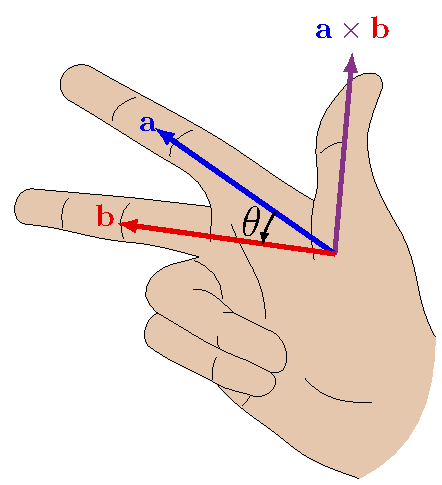
\includegraphics[width=0.2\textwidth]{src/vector/image1.pdf}
          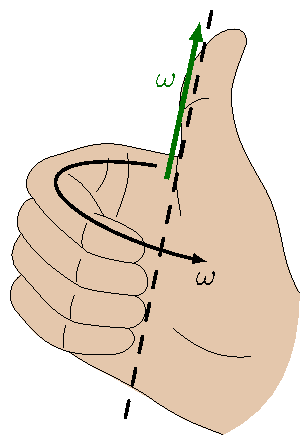
\includegraphics[width=0.15\textwidth]{src/vector/image2.pdf}
        \end{figure}
  \item \(\vec{u} \times \vec{v} \perp {\vec{u}, \vec{v}}\)
  \item \(\vec{u} \times \vec{v}\) rappresenta l'area del parallelogrammo di spigoli \(\vec{u}\) e \(\vec{v}\) (da definizione di determinante)
        \begin{figure}[H]
          \centering
          \tdplotsetmaincoords{70}{120}
          \begin{tikzpicture}[tdplot_main_coords, scale=0.5]

            % Valori massimi degli assi (puoi modificarli se necessario)
            \def\xMax{7}
            \def\yMax{7}
            \def\zMax{6}

            % Vettori u, v, w
            \def\ax{4} \def\ay{2} \def\az{0} % Vettore w
            \def\bx{0} \def\by{4} \def\bz{0} % Vettore v 
            \def\cx{0} \def\cy{1} \def\cz{3} % Vettore u
            \def\dx{0} \def\dy{0} \def\dz{5} % Vettore vxw
            % Disegno degli assi
            \draw[-latex, thick] (-\xMax,0,0) -- (\xMax,0,0) node[anchor=north east]{\(x\)};
            \draw[-latex, thick] (0,-\yMax,0) -- (0,\yMax,0) node[anchor=west]{\(y\)};
            \draw[-latex, thick] (0,0,-\zMax/2) -- (0,0,\zMax) node[anchor=south]{\(z\)};

            % Disegno del parallelepipedo 
            \coordinate (O) at (0,0,0); % Origine
            \coordinate (B) at (\ax,\ay,\az); % Punto terminale di u
            \coordinate (D) at (\bx,\by,\bz); % Punto terminale di v
            \coordinate (H) at (\cx,\cy,\cz); % Punto terminale di w
            \coordinate (M) at (\dx,\dy,\dz); % Punto terminale di v x w
            % Calcolo degli altri vertici
            \coordinate (C) at ($(B) + (D)$);
            \coordinate (E) at ($(B) + (H)$);
            \coordinate (G) at ($(D) + (H)$);
            \coordinate (F) at ($(B) + (D) + (H)$);

            % Disegno del parallelepipedo
            \draw[fill=mygray, opacity=0.3] (O) -- (B) -- (C) -- (D) -- cycle; % Faccia di base
            % Disegno dei vettori
            \draw[-stealth, ultra thick, blue]  (O) -- (B) node[anchor=north west]{\(\vec{u}\)};
            \draw[-stealth, ultra thick, red]   (O) -- (D) node[anchor=south east]{\(\vec{v}\)};
            \draw[-stealth, ultra thick, violet] (O) -- (M) node[anchor=west]{\(\vec{v} \times \vec{w}\)};
            %Disegno angolo tra u e v x w
            \tdplotsetrotatedcoords{90}{0}{0}
            \begin{scope}[tdplot_rotated_coords]
              \tdplotdrawarc[tdplot_rotated_coords, ->,thick]{(O)}{2}{0}{-60}{anchor=south}{$\theta$}
            \end{scope}
          \end{tikzpicture}
        \end{figure}
\end{itemize}

\subsubsection{Prodotto misto}
Chiamiamo \textbf{prodotto misto} di tre vettori \(\vec{u}, \vec{v}, \vec{w} \in \mathbb{R}^3\) il numero reale:
\begin{equation}
  \boxed{\vec{u} \cdot \left(\vec{v} \times \vec{w}\right) = det \begin{pmatrix}
      u_1 & u_2 & u_3 \\
      v_1 & v_2 & v_3 \\
      w_1 & w_2 & w_3
    \end{pmatrix}}
\end{equation}
\textbf{Proprietà}
\begin{itemize}
  \item \( | \vec{u} \cdot \left(\vec{v} \times \vec{w}\right) | \) rappresenta il volume del parallelepipedo di spigoli \(\vec{u}, \vec{v}, \vec{w}\), posso calcolare come \\
        \( | \vec{u} \cdot \left(\vec{v} \times \vec{w}\right) | \cdot |\cos |\hat{u \cdot (v \times w)}|| \) ,
        \begin{figure}[H]
          \centering
          \tdplotsetmaincoords{70}{120}
          \begin{tikzpicture}[tdplot_main_coords, scale=0.5]

            % Valori massimi degli assi (puoi modificarli se necessario)
            \def\xMax{7}
            \def\yMax{7}
            \def\zMax{6}

            % Vettori u, v, w
            \def\ax{3} \def\ay{0} \def\az{0} % Vettore w
            \def\bx{0} \def\by{3} \def\bz{0} % Vettore v 
            \def\cx{0} \def\cy{1} \def\cz{3} % Vettore u
            \def\dx{0} \def\dy{0} \def\dz{5} % Vettore u
            % Disegno degli assi
            \draw[-latex, thick] (-\xMax,0,0) -- (\xMax,0,0) node[anchor=north east]{\(x\)};
            \draw[-latex, thick] (0,-\yMax,0) -- (0,\yMax,0) node[anchor=west]{\(y\)};
            \draw[-latex, thick] (0,0,-\zMax/2) -- (0,0,\zMax) node[anchor=south]{\(z\)};

            % Disegno del parallelepipedo 
            \coordinate (O) at (0,0,0); % Origine
            \coordinate (B) at (\ax,\ay,\az); % Punto terminale di u
            \coordinate (D) at (\bx,\by,\bz); % Punto terminale di v
            \coordinate (H) at (\cx,\cy,\cz); % Punto terminale di w
            \coordinate (M) at (\dx,\dy,\dz); % Punto terminale di v x w
            % Calcolo degli altri vertici
            \coordinate (C) at ($(B) + (D)$);
            \coordinate (E) at ($(B) + (H)$);
            \coordinate (G) at ($(D) + (H)$);
            \coordinate (F) at ($(B) + (D) + (H)$);

            % Disegno del parallelepipedo
            \draw[fill=mygray, opacity=0.3] (O) -- (B) -- (C) -- (D) -- cycle; % Faccia di base
            \draw[fill=mygray, opacity=0.3] (E) -- (B) -- (C) -- (F) -- cycle; % Faccia laterale 1
            \draw[fill=mygray, opacity=0.3] (E) -- (B) -- (O) -- (H) -- cycle; % Faccia laterale 2
            \draw[fill=mygray, opacity=0.3] (H) -- (O) -- (D) -- (G) -- cycle; % Faccia laterale 3
            \draw[fill=mygray, opacity=0.3] (C) -- (F) -- (G) -- (D) -- cycle; % Faccia laterale 4
            \draw[fill=mygray, opacity=0.3] (E) -- (H) -- (G) -- (F) -- cycle; % Faccia superiore
            % Disegno dei vettori
            \draw[-stealth, ultra thick, blue]  (O) -- (B) node[anchor=north west]{\(\vec{w}\)};
            \draw[-stealth, ultra thick, red]   (O) -- (D) node[anchor=south east]{\(\vec{v}\)};
            \draw[-stealth, ultra thick, orange](O) -- (H) node[anchor=west]{\(\vec{u}\)};
            \draw[-stealth, ultra thick, violet] (O) -- (M) node[anchor=west]{\(\vec{v} \times \vec{w}\)};
            %Disegno angolo tra u e v x w
            \tdplotsetrotatedcoords{0}{-90}{0}
            \begin{scope}[tdplot_rotated_coords]
              \tdplotdrawarc[tdplot_rotated_coords, ->]{(O)}{2}{0}{20}{anchor=south}{$\theta$}
            \end{scope}
          \end{tikzpicture}
        \end{figure}
\end{itemize}
\subsection{Applicazione del calcolo vettoriale}
\subsubsection{Piano passante per un punto e ortogonale a un vettore}
Sia \(P_0= x_0, y_0,z_0\) un punto di \(\mathbb{R}^3\) con posizione
\begin{equation*}
  \vec{r_0}= x_0 \hat{i} + y_0 \hat{j} + z_0 \hat{k}
\end{equation*}
Sia \[\vec{n}= A \hat{i} + B \hat{j} + C \hat{k}\] un qualsiasi vettore assegnato \textit{non nullo}, allora esiste \textbf{un solo piano} passante per \(P_0\) e ortogonale a \(\vec{n}\)\\
Se \(\vec{r}\) è il vettore posizione di \(P= (x, y,z)\) del piano allora
\begin{eqnarray*}
  &\vec{P_0 P} = \vec{r} - \vec{r_0}\\
  &\vec{P_0 P} = (x - x_0) \hat{i} + (y - y_0) \hat{j} + (z - z_0) \hat{k}\\
  &\vec{P_0 P} = (x - x_0, y - y_0, z - z_0)
\end{eqnarray*}
Il piano è ortogonale\(\perp\) a \(\vec{n}\) se e solo se
\begin{equation}
  \boxed{\vec{P_0 P} \cdot \vec{n} = 0}
\end{equation}
che in forma scalare diventa
\begin{equation}
  \boxed{ \mathcal{P} : A(x - x_0) + B(y - y_0) + C(z - z_0) = 0}
\end{equation}
\begin{figure}[H]
  \centering
  \tdplotsetmaincoords{80}{120}
  \begin{tikzpicture}[tdplot_main_coords, scale=0.5]
    % Valori massimi degli assi (puoi modificarli se necessario)
    \def\xMax{7}
    \def\yMax{7}
    \def\zMax{6}



    % Coordinate del vettore n
    \def\nAx{4}
    \def\nAy{4}
    \def\nAz{7}

    % Coordinate del punto P₀
    \def\xZero{4}
    \def\yZero{4}
    \def\zZero{4}

    % Calcolo del punto P
    \def\x{4}
    \def\y{7}
    \def\z{4}

    \coordinate (A) at (3,3,4);
    \coordinate (B) at (10,3,4);
    \coordinate (C) at (10,10,4);
    \coordinate (D) at (3,10,4);

    % Disegno degli assi
    \draw[-latex, thick] (-\xMax,0,0) -- (\xMax,0,0) node[anchor=north east]{\(x\)};
    \draw[-latex, thick] (0,-\yMax,0) -- (0,\yMax,0) node[anchor=west]{\(y\)};
    \draw[-latex, thick] (0,0,-\zMax/2) -- (0,0,\zMax) node[anchor=south]{\(z\)};

    % Disegno del piano
    \fill[cyan, opacity=0.3](A) -- (B) -- (C) -- (D) -- cycle;
    %Bordo del piano
    \draw (A) -- (B) -- (C) -- (D) -- cycle;
    % Disegno dei vettori
    \draw[-stealth, ultra thick, blue]  (0,0,0) -- (\x,\y,\z) node[anchor=south west]{\(\vec{r}\)};
    \draw[-stealth, ultra thick, blue]  (0,0,0) -- (\xZero,\yZero,\zZero) node[above left]{\(\vec{r_0}\)};
    \draw[-stealth, ultra thick, red]   (\xZero,\yZero,\zZero) -- (\nAx,\nAy,\nAz) node[left]{\(\vec{n}\)};
    \draw[-stealth, ultra thick, violet] (\xZero,\yZero,\zZero) -- (\x,\y,\z) node[anchor=south east]{\(\vec{r}- \vec{r_0}\)};

    % Disegno del punto P₀
    \filldraw[black] (\xZero,\yZero,\zZero) circle (2pt) node[anchor= east]{\(P_0\)};
    % Disegno del punto P
    \filldraw[black] (\x,\y,\z) circle (2pt) node[anchor=north west]{\(P\)};

  \end{tikzpicture}

\end{figure}
\subsubsection{Distanza punto da un piano}
Sia \(\mathcal{P}\) il piano di equazione cartesiana
\begin{equation*}
  \mathcal{P} : Ax + By + Cz + D = 0
\end{equation*}
e sia
\begin{equation*}
  P_0(x_0, y_0, z_0)
\end{equation*}
un punto \(\in \mathbb{R}^3 \setminus \mathcal{P}\), sia inoltre
\begin{equation*}
  \hat{n} = A \hat{i} + B \hat{j} + C \hat{k}
\end{equation*}
un vettore normale a \(\mathcal{P}\), allora se \(P_1\) è la proiezione ortogonale di \(P_0\) su \(\mathcal{P}\) allora
\begin{equation}
  \boxed{d(P_0, \mathcal{P}) = |P_0 P_1| = \frac{|Ax_0 + By_0 + Cz_0 + D|}{\sqrt{A^2 + B^2 + C^2}}}
\end{equation}

\newpage
\subsection{Derivate}
\subsubsection{Derivate parziali}
Sia \(f : A \subseteq \mathbb{R}^2 \rightarrow \mathbb{R}\) una funzione di due variabili, allora la derivata parziale di \(f\) rispetto a \(x\) in \((x_0, y_0)\) è
\begin{equation}
  \boxed{
    \frac{\partial f}{\partial x} (x_0, y_0) = f_x(x_0, y_0) = \lim_{h \to 0} \frac{f(x_0 + h, y_0) - f(x_0, y_0)}{h}
  }
\end{equation}
mentre la derivata parziale di \(f\) rispetto a \(y\) in \((x_0, y_0)\) è
\begin{equation}
  \boxed{
    \frac{\partial f}{\partial y} (x_0, y_0) = f_y(x_0, y_0) = \lim_{h \to 0} \frac{f(x_0, y_0 + h) - f(x_0, y_0)}{h}
  }
\end{equation}
\paragraph[short]{Esempio}
Sia \(f(x, y) = x^2 + y^2\), allora
\begin{equation*}
  \frac{\partial f}{\partial x} = 2x \quad \frac{\partial f}{\partial y} = 2y
\end{equation*}
\subsubsection{Gradiente}
Il gradiente di una funzione \(f : A \subseteq \mathbb{R}^2 \rightarrow \mathbb{R}\) è il vettore
\begin{equation}
  \boxed{
    \nabla f =  \left(\frac{\partial f}{\partial x}, \frac{\partial f}{\partial y}\right) = \left(f_x, f_y\right)
  }
\end{equation}
\paragraph[short]{Esempio}
Sia \(f(x, y) = x^2 + y^2\), allora
\begin{equation*}
  \nabla f = \left(2x, 2y\right)
\end{equation*}
\subsubsection{Derivate direzionali}
Sia \(f : A \subseteq \mathbb{R}^2 \rightarrow \mathbb{R}\) una funzione di due variabili, allora la derivata direzionale di \(f\) in \((x_0, y_0)\) lungo il vettore \(\vec{v} = v_1 \hat{i} + v_2 \hat{j}\) è
\begin{equation}
  \frac{\partial f}{\partial \vec{v}} (x_0, y_0) = \nabla f \cdot \vec{v} = f_x(x_0, y_0) \cdot v_1 + f_y(x_0, y_0) \cdot v_2
\end{equation}
\paragraph[short]{Esempio}
Sia \(f(x, y) = x^2 + y^2\), e \(\vec{v} = \left(1, 1\right)\), allora
\begin{equation*}
  \nabla f = \left(2x; 2y\right) \quad \nabla f \cdot \vec{v} = 2x + 2y
\end{equation*}
\end{document}



\subsection{Limiti e continuità per funzioni di più variabili}
Stiamo operando con le funzioni del tipo
\begin{equation*}
  f: A \subseteq \mathbb{R}^n \rightarrow \mathbb{R}
\end{equation*}
\subsubsection{Intorni sferici}
Dato \(\vec{x}_0 \in \mathbb{R}^n\), chiamiamo \textbf{intorno sferico} di centro \(\vec{x}_0\) e raggio \(r > 0\) l'insieme
\begin{equation}
  U_r(\vec{x}_0) = \left\{\vec{x} \in \mathbb{R}^n : |\vec{x}-\vec{x}_0| <r \right\}
\end{equation}
per qualche \(r > 0\), che si dice \textbf{raggio dell'intorno}; \(x_0\) si dice \textbf{centro dell'intorno}.\\
\subsubsection{Derivato}
Se \(A \subseteq \mathbb{R}^n\), diremo che \(\vec{x}_0\) è \textbf{di accumulazione} per \(A\), se \(\forall r > 0\) l'insieme :
\begin{equation*}
  U_r (\vec{x_0}) \cap A \setminus \{\vec{x}_0\} \neq \emptyset
\end{equation*}
l'insieme dei punti di accumulazione per \(A\) scritto \(D(A)\), detto \textbf{derivato} di \(A\).
\subsubsection{Limite finito}
Sia \(f : A \rightarrow \mathbb{R}\), \(\vec{x}_0 \in D(A), L \in \mathbb{R}\) è il \textbf{limite} per \(\vec{x}\) che tende a \(\vec{x_0}\) in \(A\) e scriviamo
\begin{equation}
  \lim_{\substack{\vec{x} \rightarrow \vec{x}_0 \\ x \in A }} f(\vec{x}) = L
\end{equation}
, se
\begin{equation*}
  \forall \varepsilon >0 \exists \delta(\varepsilon) > 0 \text{ t.c. } \mid f(\vec{x}) - L \mid\  \leq \varepsilon\ \forall \vec{x} \in  \biggl( U_{\delta(\varepsilon)}(\vec{x}_0) \cap A \biggr) \setminus \biggl\{\vec{x}_0\biggr\}
\end{equation*}

\subsubsection{Limite infinito}
Si dice che \(f\) ha limite \(+\infty \lor -\infty\), e si scrive
\begin{equation}
  \lim_{\substack{\vec{x} \rightarrow \vec{x}_0 \\ x \in A }} f(\vec{x}) = +\infty \lor -\infty
\end{equation}
, se
\begin{equation*}
  \forall k > 0\ \exists\ \delta(k) > 0 \text{ t.c } f(\vec{x})>k \lor f(\vec{x})<k
\end{equation*}

\subsubsection{Continuità}
Se \(\vec{x}_0 \in A \cap D(A)\) diremo che \(f\) è \textbf{continua} in \(\vec{x}_0\) se
\begin{equation}
  \lim_{\substack{\vec{x} \rightarrow \vec{x}_0 \\ \vec{x} \in A }} f(\vec{x}) = f(\vec{x}_0)
\end{equation}
Se \(\vec{x}_0 \in A \setminus D(A)\), ossia è isolato, allora \(f\) è \textbf{continua} in \(\vec{x}_0\) \\
Segue che se \(f : A \rightarrow \mathbb{R}^m\), \(\vec{x}_0 \in \cap D(A)\), allora \(f\) è \textbf{continua} in \(\vec{x}_0\) se e solo se tutte le sue componenti sono continue in \(\vec{x}_0\), ossia
\begin{equation}
  \lim_{\substack{\vec{x} \rightarrow \vec{x}_0 \\ \vec{x} \in A }} \vec{f}(\vec{x}) = \vec{f} (\vec{x}_0) = \lim_{\substack{\vec{x} \rightarrow \vec{x}_0 \\ \vec{x} \in A }} f_i (\vec{x}) = f_i (\vec{x}_0)
\end{equation}
\subsection{Teoremi validi per funzioni di più variabili}
Per le funzioni di più variabili \(f : A \subseteq \mathbb{R}^n \rightarrow \mathbb{R}\) valgono quasi tutti i teoremi visti per le funzioni di una variabile
\subsubsection{Teorema di permanenza del segno}
Sia \(f: A \subseteq \mathbb{R}^n \rightarrow \mathbb{R}\), \(\vec{x}_0 \in D(A)\), se
\begin{equation*}
  \lim_{\substack{\vec{x} \rightarrow \vec{x}_0 \\ x \in A }} f(\vec{x}) = L \in \mathbb{R}
\end{equation*}
allora
\begin{enumerate}
  \item se \(L > 0 \), \(\exists\ r > 0 \) t.c. \(f(\vec{x}) > 0 \) in \(\bigl(U_r(\vec{x}_0) \cap A\bigr) \setminus \bigl\{\vec{x}_0\bigr\}\)
  \item se \(f\geq 0\) in \(U_r(\vec{x}_0) \cap A \setminus \bigl\{\vec{x}_0\bigr\}\), per qualche \(r > 0\), allora \(L \geq 0\)
  \item se \(f\) è continua in \(\vec{x}_0 \in A \cap D(A)\) e \(f(\vec{x}_0) > 0 \), allora \(\exists\ r > 0 \) t.c. \(f(\vec{x}) > 0 \) in \(\bigl(U_r(\vec{x}_0) \cap A\bigr)\)
\end{enumerate}

\newpage

\section{Esercizio esame}

\textbf{Condizioni di esistenza per l'equazione vettoriale}

Consideriamo l'equazione vettoriale:

\[
  \mathbf{a} \times \mathbf{x} = \mathbf{b}
\]

dove $\mathbf{a}, \mathbf{b} \in \mathbb{R}^3 \setminus \{0\}$ e sono vettori fissati. Dimostrare che l'equazione ha una soluzione se e solo se il vettore $\mathbf{b}$ è ortogonale al vettore $\mathbf{a} \times \mathbf{b}$.

\textbf{Soluzione:}

\begin{enumerate}
  \item \textbf{Condizione di ortogonalità:}

        Calcoliamo il prodotto scalare tra $\mathbf{a} \times \mathbf{x}$ e $\mathbf{a}$:

        \[
          (\mathbf{a} \times \mathbf{x}) \cdot \mathbf{a} = \mathbf{a} \cdot (\mathbf{a} \times \mathbf{x})
        \]

        Per la proprietà del prodotto vettoriale, $\mathbf{a} \cdot (\mathbf{a} \times \mathbf{x}) = 0$. Sostituendo $\mathbf{a} \times \mathbf{x}$ con $\mathbf{b}$, otteniamo:

        \[
          \mathbf{b} \cdot \mathbf{a} = 0
        \]

        Quindi, il vettore $\mathbf{b}$ è ortogonale al vettore $\mathbf{a}$.

  \item \textbf{Dimostrazione della necessità:}

        Supponiamo che l'equazione $\mathbf{a} \times \mathbf{x} = \mathbf{b}$ abbia una soluzione $\mathbf{x}$. Per la proprietà del prodotto vettoriale, $\mathbf{b} \cdot \mathbf{a} = 0$, come dimostrato sopra.

  \item \textbf{Dimostrazione della sufficienza:}

        Supponiamo che $\mathbf{b}$ sia ortogonale a $\mathbf{a}$, ovvero $\mathbf{b} \cdot \mathbf{a} = 0$. Consideriamo un vettore $\mathbf{x}$ tale che:

        \[
          \mathbf{x} = \lambda \mathbf{a} + \mathbf{y}
        \]

        dove $\lambda$ è un numero reale e $\mathbf{y}$ è un vettore qualsiasi ortogonale a $\mathbf{a}$. Calcoliamo il prodotto vettoriale $\mathbf{a} \times \mathbf{x}$:

        \[
          \mathbf{a} \times \mathbf{x} = \mathbf{a} \times (\lambda \mathbf{a} + \mathbf{y}) = \lambda (\mathbf{a} \times \mathbf{a}) + \mathbf{a} \times \mathbf{y}
        \]

        Per la proprietà del prodotto vettoriale, $\mathbf{a} \times \mathbf{a} = \mathbf{0}$. Inoltre, $\mathbf{a} \times \mathbf{y}$ è ortogonale a $\mathbf{a}$ perché $\mathbf{y}$ è ortogonale a $\mathbf{a}$. Quindi, $\mathbf{a} \times \mathbf{x} = \lambda \mathbf{0} + \mathbf{b} = \mathbf{b}$.

        Ciò dimostra che se $\mathbf{b}$ è ortogonale a $\mathbf{a}$, l'equazione $\mathbf{a} \times \mathbf{x} = \mathbf{b}$ ha una soluzione.

\end{enumerate}

\textbf{Conclusione:}

L'equazione $\mathbf{a} \times \mathbf{x} = \mathbf{b}$ ha una soluzione se e solo se il vettore $\mathbf{b}$ è ortogonale al vettore $\mathbf{a} \times \mathbf{b}$.

\textbf{Casi notevoli:}

\begin{itemize}
  \item Se $\mathbf{a} = \mathbf{0}$, l'equazione non ha soluzioni per nessun $\mathbf{b}$.
  \item Se $\mathbf{b} = \mathbf{0}$, l'equazione ha infinite soluzioni, perché qualsiasi vettore $\mathbf{x}$ è soluzione.
\end{itemize}

\textbf{Applicazioni:}

Questa proprietà è utile in diverse applicazioni, come la geometria computazionale e la fisica, dove è necessario trovare il punto di intersezione tra due rette o piani.
